\documentclass{article}
\usepackage[utf8]{inputenc}
\usepackage{graphicx}

\begin{document}
    \begin{titlepage}
 \begin{sffamily}
  \begin{center}
            
\includegraphics[scale=0.04]{Images/ubx-logo.png}
            \\[2cm]
        
    
    {\huge \bfseries  Projet de Programmation : CoreWar \\ Cahier des besoins\\ [0.5cm] }

    \rule{\linewidth}{.5pt}
    \\[2cm]

    \begin{minipage}{0.4\textwidth}
      \begin{flushleft} \large
        \author{}Étudiants : \item Frédéric Chipot \item Florian Dayre \item Louis Duplantier \item Alex Fournier \item Gaël Halnaut
            
      \end{flushleft}
    \end{minipage}
    \begin{minipage}{0.4\textwidth}
      \begin{flushright} \large
        \emph{}\\  \textsc{}
      \end{flushright}
    \end{minipage}

    \vfill

    {\large \today}

  \end{center}
  \end{sffamily}
  
\end{titlepage}

\section{Introduction}
    \paragraph{} Ce projet de programmation porte sur le thème de CoreWar. CoreWar est un jeu de contrôle d'espace mémoire, dont l'objectif est d'être le dernier survivant et prendre le  contrôle de la mémoire ! Le jeu se déroule selon le schéma  suivant : chaque joueur propose un programme (ici une liste d'instructions en langage assembleur, le redCode) qui constitue son combattant. Ces programmes vont s'affronter (s'exécuter) sur une machine virtuelle, MARS (Memory Array Redcode Simulator), dans une mémoire commune. Lorsqu'un programme est sur une case mémoire, il exécute son contenu et passe sur la case suivante (sauf contre indication de l'instruction). Si la case sur laquelle il se trouve n'est pas composée d'instruction mais de données (bombe), le programme meurt. 

    \paragraph{} Dans ce projet l'objectif principal va être de générer des guerriers grâce à un algorithme d'évolution. Afin de suivre l'évolution des guerriers générés nous avons comme objectif secondaire de développer un outil facilitant des modifications future ainsi que l'optimisation des performances des guerriers. Il faudrait que cet outil puisse à long terme stocker les données suivantes : répertorier les différents guerriers, l'historique de leurs modifications et un indicatif (moyenne par exemple) de leurs performances une fois les modifications faites. Ces options permettraient aux utilisateurs de visualiser clairement l'avancée de l'algorithme d'évolution. Nous nous baserons sur la capacité des guerriers à vaincre la majorité des ennemis (pas nécessairement les plus puissants) afin d'évaluer l'efficacité des guerriers produits. 


\section{Les besoins}
    \subsection{Les besoins fonctionnels}
        \subsubsection{Pour le système}
            \begin{itemize}
                \item Développer un système de score à l'aide d'un algorithme qui attribuera un score à un guerrier à la fin d'un combat. Il y a tout un tas de raisons que tel guerrier ait pu perdre qui ne sont pas reliées directement à ses performances(position, les ennemis, leur nombre, leurs caractéristiques...), il est possible qu'avec une configuration légèrement différente, les résultats auraient été différents. Une victoire attribue un score de 1 au guerrier. Les résultats seront par contre plus nuancés pour les défaites selon les actions du guerrier. Si ce dernier est parvenu à accomplir des objectifs particulier (s'accaparer une partie de la mémoire, rester "en vie" un certain temps, l'action d'avoir vaincu d'autres guerriers, ou d'avoir survécu jusqu'à la fin en cas d'égalité, etc...) avec une valeur x comprise entre 0 et 1.
                \item Développer un algorithme d’évolution pour créer nos guerriers : Pour cela nous avons à notre disposition un document présentant une sorte d'algorithme d'évolution. Nous allons donc pouvoir partir de cela et le modifier pour essayer de le rendre plus performant.
                \begin{itemize}
                    \item Entrée : Rien ou une moyenne des résultats des derniers combats.
                    \item Sortie : La nouvelle génération N de guerriers
                    \item Contraintes :  
                        \begin{itemize}
                            \item Cet algorithme devra s'exécuter pour un nombre de fois indiqué à l'avance, représentant le nombre de générations de guerriers qu'il pourra créer. Ce nombre devra être fixé suivant une contrainte de temps d'exécution.
                            \item Il faudra également indiquer le nombre de guerriers qu'il devra créer pour une génération ainsi que les différents paramètres du tournoi sur MARS.
                        \end{itemize}
                \end{itemize}
                \item Développer un algorithme qui fait s’affronter nos guerriers dans MARS et récupère les résultats :
                \begin{itemize}
                    \item Entrée : Les guerriers de la génération N
                    \item Sortie : les résultats du combat ou d’une série de combats dans MARS
                \end{itemize}
                \item Créer un groupe de guerrier d’évaluation pour évaluer les performances finales de l’algorithme d’évolution de manière stable (= génération N0)
            \end{itemize}

    \subsubsection{Pour l'utilisateur}
        \begin{itemize}
            \item Développer un outil qui répertorie visuellement notre avancé sur l’algorithme d’évolution (réf Figure 1, page 4) :
            \begin{itemize}
                \item Entrée : La génération de l’algorithme d’évolution, Les paramètres utilisés, les résultats obtenus par les guerriers créés par cette algorithme
                \item Sortie : Interface graphique sous forme de graphe avec comme "noeuds" les différentes générations d'algorithme d'évolution et comme "arêtes" les liens existants entre les divers algorithmes.
            \end{itemize}
        \end{itemize}
\newpage
             \begin{figure}
                \centerline{\includegraphics[scale=0.5]{Images/Schéma_Outil_Versionning.png}}
                \caption{Exemple de sortie de notre outil de gestion des versions de notre algorithme d'évolution} 
            \end{figure}
\newpage
           
            
    \subsection{Ressources}
        \begin{itemize}
            \item Nous avons besoin d'un environnement sur lequel peut s'exécuter MARS, un PC simple suffit à la tâche. 
            \item Nous avons également besoin de nombreux guerriers avec lesquels on puissent comparer les performances des guerriers engendrés par l'algorithme d'évolution. Le code de nombreux guerriers est disponible en ligne, cela ne posera pas de problèmes. 
        \end{itemize}
    \subsection{Les besoins non-fonctionnels}
        \begin{itemize}
            \item Les guerriers et la méthode employée pour les créer doivent être le plus efficace possible. Le guerrier ne doit pas forcément gagner contre les meilleurs mais doit le faire le plus souvent possible. Doit proposer un guerrier final le plus rapidement possible.
            \item Clarté et facilité de compréhension de l’évolution de notre algorithme et de nos guerriers via un outil : 
            \begin{itemize}
                \item Représentation sous forme de graphe pour visualiser les liens entre les différents algorithmes 
                \item Aperçu et comparaison rapide de deux versions
            \end{itemize}
        \end{itemize}
            \begin{figure}
                \centerline{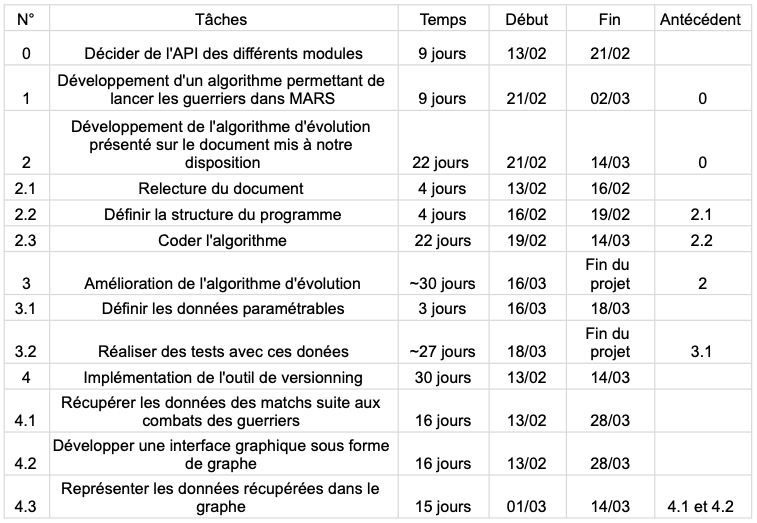
\includegraphics[scale=0.7]{Images/Gantt.png}}
                \caption{Diagramme de Gantt du projet} 
            \end{figure}
\end{document}
